
\section{Procedures}
\label{cp6:procedures}



In this section, we detail the instructions provided to the participants so that 
they could perform our experiment. 
First, we present an overview of the whole experiment and then, we detail
instructions specific to the manual and tool-assisted tasks, respectively.



The entry point to our experiment was the advertisement email.
The email disclosed the purpose of the experiment, eligibility criteria, an estimate of the time that one would take to complete the study as well as a link 
to a web survey containing the experiment's consent form and tasks. 


Once a participant consented to participate, the survey gathered demographics and then, 
it gave participants further instructions 
about how to perform each task, requesting them to install the study tool, a web browser plug-in.
Setup was followed by a short practice task---separate from the experimental tasks---that allowed participants to familiarize themselves with the content of a task, the tool, and the coding environment that we used (Colab). 


Once a participant completed the practice task, the survey randomly assigned to them a \textit{manual} task, which was followed by a randomly assigned \textit{tool-assisted} tasks---different from the manual task. While tasks were randomly assigned, we made sure that an even number of participants attempted a task with and without tool support.
For each task, including the practice tasks, the survey provided to the participants a link 
to the task description (Figure~\ref{fig:nytimes-task-github}) and asked them to submit a solution for the task, i.e., written Python code. 


Once a participant submitted their solutions, the survey
asked them about any additional feeback that they wished to share and 
offered them the opportunity to enter a raffle for one of two iPads 64 GB 
to compensate them for their time, what concluded the experiment.



\subsection{Manual Task}
\label{cp6:procedures-manual}



In the \textit{manual} task, we use the study tool to gather text that a participant deems useful for the task at hand. In this task, 
the survey asked participants to use the study tool to highlight sentences that they deemed useful and that provided information that assisted task completion---instructions similar to the ones used for the creation of the \acs{DS-android} corpus (Section~\ref{cp4:corpus-relevant-text}).



Figure~\ref{fig:artifact-pre-highlight}
gives insight into how participants highlighted sentences using the study tool. 
Whenever a participant inspected one of the artifacts available for their task, 
they could click on the \texttt{highlight} button in the tool's context menu.  
This would then instrumented the HTML of the page identifying individual sentences. 
A participant could hover over identified sentences and select them as relevant by clicking on the hovered text.
Once a participant had finished selecting sentences, they could submit 
their data also through the tool's context menu.


% As an example, Figure~\ref{fig:artifact-pre-highlight} shows a sentence discussing the \texttt{find\_all} method, which 
% one of the participants in our experiment deemed 
% relevant to the \texttt{NYTimes} task.
% Based on the pilots, we observed that the most natural flow adopted by participants was to highlight text on-the-fly. That is, they indicated what text 
% was relevant for the task at hand while they consulted each artifact and wrote their solution. 



\begin{figure}
    \centering
    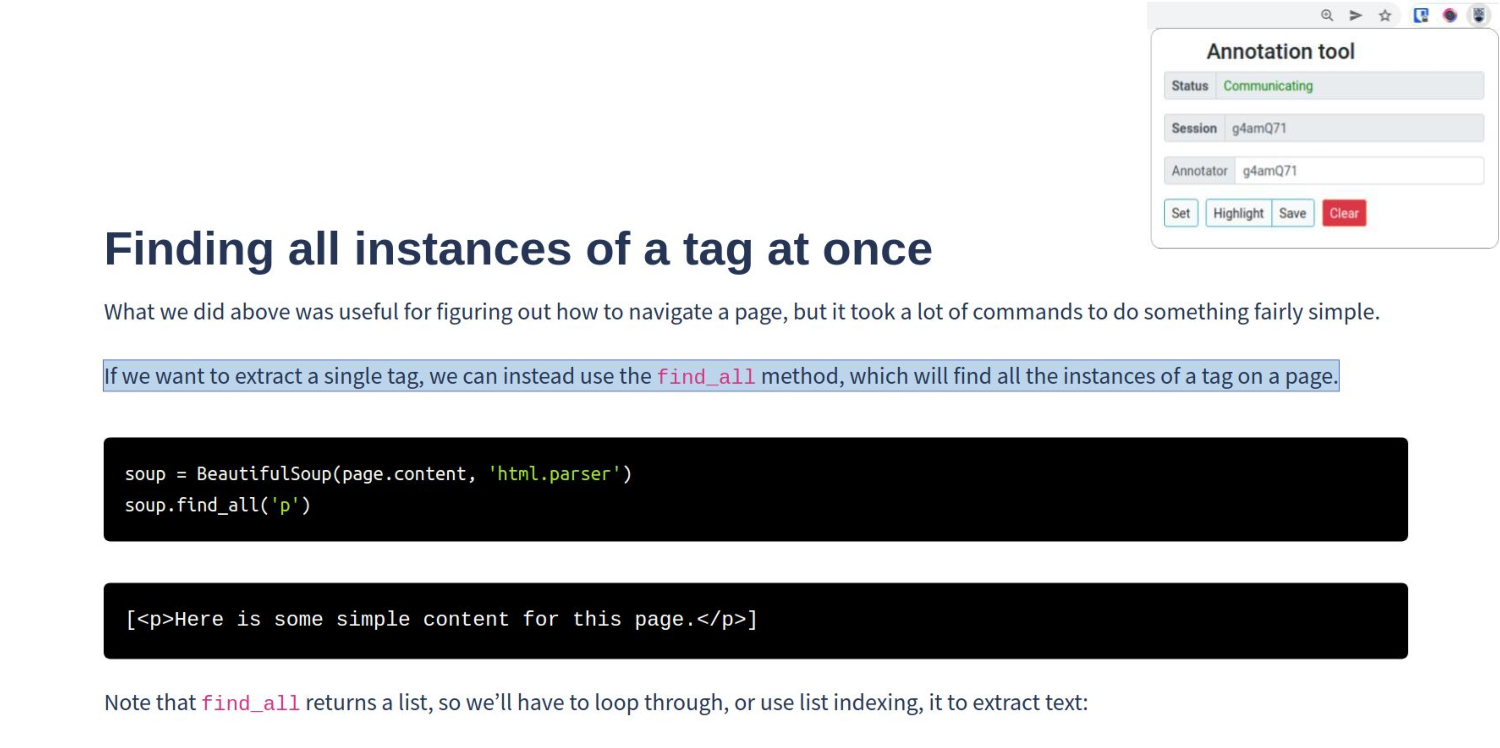
\includegraphics[width=0.95\textwidth]{cp6/manual-task.pdf}
    \caption{\texttt{BeautifulSoup} web tutorial showing the study's tool context menu (top-right corner) and a hovered over sentence}
    \label{fig:artifact-pre-highlight}
\end{figure}




\subsection{Tool-assisted Task}
\label{cp6:procedures-tool-assisted}


In the tool-assisted task, the study tool automatically highlighted text that 
its underlying semantic-based approach identified as relevant to the participant's task.
For that, the tool applies the \texttt{BERT} technique with no filters (Chapter~\ref{ch:identifying}),
automatically identifying a target number of sentences equal to 10\% of the entire content of an input artifact up to a maximum of 10 sentences per artifact.
These sentences are then highlighted in a format similar to the one in Figure~\ref{fig:artifact-pre-highlight}, but without the need for any actions by a participant.





For this task, when a participant submitted their solution, we asked them to 
rate in a 5 points Likert scale~\cite{likert1932technique} how helpful were the highlights shown by the tool.
Figure~\ref{fig:experiment-rating} shows an example of how we gathered data about the usefulness of the text automatically identified.
Participants rated highlights on a per artifact basis. A hyperlink also let a participant 
revisit an artifact and its highlights before giving their answer.
We decided to gather input at the artifact level because it would be too exhausting for a participant 
to provide individual feedback on each highlight shown.



% Our tool did not more than determine what tool-assisted task was being performed 
% and highlight the text in an artifact under inspection.
% To determine what text was relevant to a task in a certain artifact, we applied one of the most promising semantic-based techniques that we have explored in Chapter~\ref{ch:identifying}, i.e., \texttt{BERT} with no filters,
% taking the techniques output and using our web browser tool to highlighting the text identified.
% As a proof of concept, we decided to pre-cache the output 
% for the text automatically identified in each of the tasks and artifacts in our experiment. 



% Although we evaluate the usefulness of all the highlights for a task
% aggregating individual responses, we use the ratings per artifact to explore if the highlights shown in a certain type or artifact, e.g., API documents or tutorials, were considered more or less useful.


\begin{figure}
\begin{mdframed}[backgroundcolor=gray!15] 
\begin{scriptsize}

\noindent \textbf{1.} Indicate whether you agree with the following statement:

\medskip

\quad \textit{The highlights in \textcolor{steelblue}{``How to extract HTTP response body from a Python requests call''} were helpful to} 

\quad \textit{correctly accomplish the task in question.}  \smallskip

\smallskip

\quad \quad \textit{(Strongly disagree)} ~$1$ - $2$ - $3$ - $4$ - $5$ ~\textit{(Strongly agree)} 


\bigskip


\noindent \textbf{2.} Indicate whether you agree with the following statement:

\medskip

\quad \textit{The highlights in \textcolor{steelblue}{``BeautifulSoup tutorial: Scraping web pages with Python''} were helpful to} 

\quad \textit{correctly accomplish the task in question.}  \smallskip

\smallskip

\quad \quad \textit{(Strongly disagree)} ~$1$ - $2$ - $3$ - $4$ - $5$ ~\textit{(Strongly agree)} 

\centering 

...

\end{scriptsize}
\end{mdframed}
\caption{Questions asking a participant to rate the usefulness of the highlights shown in two artifacts; by clicking on the name of an artifact, a participant could revisit the highlights of that artifact}
\label{fig:experiment-rating}
\end{figure}

    



\subsection{Summary of procedures}


Throughout the past sections, we have described experimental procedures 
where participants attempted a \textit{manual} and a \textit{tool-assisted}.
These procedures allowed us to gather:


\begin{enumerate}
\item a participant's submitted solution (written Python code) for each task;
\item text that participants deemed relevant for completing a manual task;
\item the usefulness of the highlights shown in a tool-assisted task; and
\item any additional feedback (written text) that a participant wished to provide.
\end{enumerate}


We use this data to investigate whether 
a tool embedding a semantic-based technique helps developers complete a software task. 


\clearpage


